\documentclass{standalone}
\usepackage[utf8]{inputenc}
\usepackage{tikz}

\usetikzlibrary{decorations, decorations.pathreplacing, decorations.pathmorphing}

\begin{document}

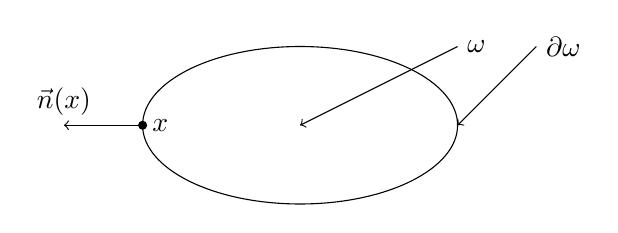
\begin{tikzpicture}
    \draw (0,0) ellipse (2cm and 1cm);
    \draw[ <-] (0,0) -- (2,1) node[right]{$\omega$};
    \draw[ <-] (2,0) -- (3,1) node[right]{$\partial\omega$};
    \draw[ ->] (-2,0) -- (-3,0) node[above]{$\vec{n}(x)$};
    \draw[fill=black] (-2,0) circle (0.05) node[right]{$x$};
\end{tikzpicture}

\end{document}
